% Hepta
\begin{figure}[H]
\centering
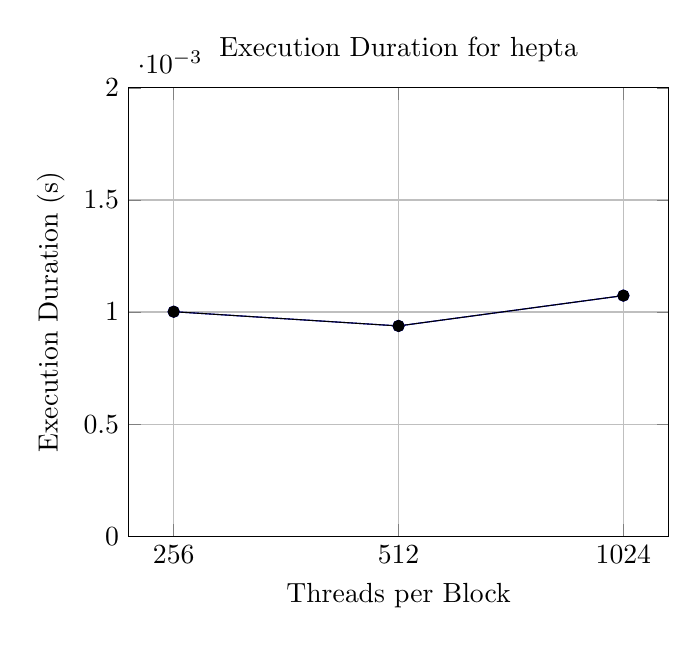
\begin{tikzpicture}
    \begin{axis}[
        xlabel={Threads per Block},
        ylabel={Execution Duration (s)},
        symbolic x coords={256, 512, 1024},
        xtick=data,
        ymin=0, ymax=0.002,
        grid=major,
        title={Execution Duration for hepta}
    ]
        \addplot coordinates {(256,0.00100147) (512,0.000937984) (1024,0.00107334)};
        \addplot[mark=*] coordinates {(256,0.00100147) (512,0.000937984) (1024,0.00107334)};
    \end{axis}
\end{tikzpicture}
\caption{Comparison of execution duration for the dataset Hepta: N212 with different
threads per thread block. Experiments are conducted on an NVIDIA RTX4070 consumer GPU}
\end{figure}